\chapter{基于同步内存回收的内存压力量化算法的设计与实现}
\label{chap:基于同步内存回收的内存压力量化算法的设计与实现}
本章详细介绍了基于同步内存回收延迟的内存压力量化算法的设计与实现细节。首先分析了同步回收延迟与内存压力的关联性,然后提出了基于同步回收延迟的内存压力量化算法的设计思想,关键技术细节,最后介绍了该算法的实现细节。

\section{同步内存回收延迟与内存压力的关联性建模}

在内存管理研究中,工作集估计算法作为核心组件,其精确性直接影响内存分配策略与页面置换决策的效能。如\ref{sec:工作集估计算法研究历史与现状}节所述,现有工作集估计方法可归纳为三类典型范式:基于统计采样的近似计算模型、依托系统运行时特征的启发式预测算法,以及基于机器学习模型的离线训练-在线预测框架。然而,机器学习算法在面对新型应用场景时存在泛化能力不足的问题,其预测性能有待进一步验证。

基于统计特征的启发式算法因其固有的运行时特性适配优势,在动态内存管理场景中展现出较高的实时性表现。其中,内存压力指标作为反映系统资源稀缺程度的量化表征,为实现高效内存卸载提供了关键的决策依据。当前研究实践中,内存压力可通过多维统计特征进行建模,包括但不限于缺页中断频率、页面分配速率等特征。通过对这些特征的线性组合分析,可构建工作集大小的近似估计模型。但现有方法在理论建模层面存在以下根本性缺陷:

\begin{itemize}
    \item 内存压力指标与工作集大小的函数关系呈现显著的非线性特征。例如,工作集转换可能导致大量缺页中断,从而干扰算法对工作集大小的准确判断。
    \item 内存压力指标未充分考虑异构存储设备在性能上的显著差异。以机械硬盘与NVM为例,二者可能发生相同次数的缺页中断,但其处理压力存在显著差异。由于NVM能够快速处理缺页中断,在不影响性能的前提下,可适当缩小工作集以节约内存资源。
\end{itemize}

本研究基于Linux内核同步内存回收机制提出新型压力度量指标,其数学表征为:
\begin{equation}
    \label{eq:mem_pressure}
    mem_pressure = \frac{T_{sync}}{T_{epoch}}
\end{equation}

其中\(T_{sync}\)表示同步回收周期耗时,\(T_{epoch}\)为监控时间窗口。

该内存压力指标的提出基于以下理论分析:当内存资源趋近瓶颈时,同步回收过程需遍历更多候选页面,导致\(T_{sync}\)呈现超线性增长特性。同时,该指标通过时间维度归一化处理,可有效消除异构卸载后端由于绝对性能差异带来的度量偏差。

\section{基于同步内存回收延迟的内存压力量化算法}
\label{sec:基于同步内存回收延迟的内存压力量化算法}

在 \ref{sec:直接页面回收机制} 节中,已经对 Linux 内核同步内存回收机制做了详细的分析,分析表明,函数\_\_alloc\_pages\_direct\_reclaim 的执行时间是反映同步回收延迟的重要指标。基于此,本章提出了一种内存压力检测方法。该方法利用内核插桩技术,在 \_\_alloc\_pages\_direct\_reclaim 函数的入口和出口处改变状态,然后在内核中每次发生同步中断的时候去更新累计时间和cpu的非空闲时间,从而直接获取每次同步回收操作的耗时。为了综合反映多 CPU 系统中不同核心的负载差异,本研究引入了多 CPU 加权聚合策略。此外,为了平滑压力数据、减少短期波动的影响,本研究采用了指数移动平均算法。此外,还采用了定点数优化技术,显著提高了计算效率。

\subsection{多核加权聚合}

本研究通过插桩技术得到是单个核心的同步回收延迟时间 \(T_c^{block}\),需要将多个核心的 \(T_c^{block}\) 聚合为一个压力值。然而,采用简单的算术平均方法计算系统压力:
\begin{equation}
    Pressure_{simple} = \frac{\sum_{c=1}^{n} T_c^{block}}{\Delta T \times n} \times 100\%
\end{equation}

其中,\(\Delta T\) 为采样周期,\(n\) 为处理器核心数量,该方法存在显著的理论缺陷,无法准确反映系统的真实内存压力状况。

首先,简单平均算法未能有效处理处理器核心负载不均衡问题。考虑一个多核系统,其中部分处理器核心处于高负载状态,而另一些核心处于空闲或低负载状态。当空闲核心上发生短暂的同步内存回收事件时,其对应的  也会被计入总和。例如,在一个四核系统中,假设一个高负载核心因内存压力产生了 0.5s 的阻塞时间,而一个空闲核心仅因参与全局同步产生了 0.1s 的阻塞时间。根据简单平均算法,系统压力将被计算为:
\[
Pressure_{simple} = \frac{0.5 + 0.1 + 0 + 0}{1.0 \times 4} \times 100\% = 15\%
\]

该结果显著低估了实际系统压力,因为将空闲核心的数据纳入计算,稀释了高负载核心所反映的真实内存压力。这种现象可定义为"空闲核心稀释效应",导致系统压力评估结果失真。

其次,简单平均算法无法准确反映不同处理器核心对系统整体性能的差异性贡献。在实际系统中,各处理器核心的负载分布往往呈现显著差异,部分核心可能长时间处于高负载状态,而其他核心则可能大部分时间处于空闲状态。简单平均算法平等对待每个核心的延迟时间,忽略了它们对系统整体性能影响的权重差异。例如,在一个双核系统中,若核心0的压力为 80\%(非空闲时间 80ms),核心1的压力为 20\%(非空闲时间 20ms),简单平均算法将得出 50\% 的系统压力。该结果未能体现核心0作为主要负载承担者的关键作用。

为克服上述缺陷,本研究提出采用加权聚合算法,该算法的核心思想是:根据每个处理器核心的运行时间分配权重。核心的运行时间越长,表明其在采样周期内处理的任务越多,其上发生的同步内存回收事件对系统整体性能的影响也越显著,他的行为也更具有代表性。 加权聚合算法的计算公式如下:

\begin{equation}
    Pressure_{weighted} = \frac{\sum_{c=1}^{n} (T_c^{block} \times W_c)}{\sum_{c=1}^{n} W_c} \times 100\%
\end{equation}

其中,\(T_c^{block}\) 表示核心 \(c\) 在采样周期 \(\Delta T\) 内的同步内存回收总延迟时间,\(W_c\) 表示核心 \(c\) 的权重,即其在采样周期 \(\Delta T\) 内的非空闲时间。分母中的 \(\sum_{c=1}^{n} W_c\) 表示所有核心的非空闲时间总和。通过这种加权方式,算法能够有效降低或消除空闲核心的"噪声"影响,同时更准确地反映不同核心负载对系统整体性能压力的贡献,从而提供更可靠、更具代表性的内存压力评估结果。

\subsubsection{指数移动平均算法}

在获取基于处理器核心的非空闲时间加权的内存压力指标后,本研究进一步考虑压力数据的平滑性以及长期趋势的分析。原始的压力数据(无论是简单平均还是加权平均)可能会因为短暂的、偶然的事件而产生剧烈波动,这些波动可能会掩盖真实的压力趋势。因此,需要采用一种有效的方法对压力数据进行平滑处理,以减少短期波动的影响,同时保留长期趋势信息。指数移动平均(Exponential Moving Average, EMA)算法\citing{https://doi.org/10.1002/for.3980040103}是满足这一需求的有效工具。

EMA 算法的核心思想是对新旧数据进行加权平均,但与简单算术平均赋予所有数据相同权重不同,EMA 赋予旧数据的影响随时间推移呈指数衰减。这种处理方式更符合实际系统的运行特征:最近发生的事件对当前系统状态的影响通常更大,而较早发生的事件的影响则逐渐减弱。具体来说,EMA 的计算公式为:
\begin{equation}
    EMA_{new} = EMA_{old} \times \alpha + P_{current} \times (1 - \alpha)
    \label{eq:EMA}
\end{equation}


其中,\(EMA_{new}\) 和 \(EMA_{old}\) 分别代表当前时刻和上一时刻的 EMA 值,\(P_{current}\) 是当前时刻的压力值,\(\alpha\) 是一个介于 0 和 1 之间的衰减因子(也称平滑因子)。衰减因子 \(\alpha\) 决定了旧数据影响力衰减的速度,也即决定了 EMA 对历史数据的"记忆"长度。它的值由采样间隔 \(\Delta T\) 和时间窗口 \(\tau\) 共同决定,关系式为:
\[
\alpha = e^{-\Delta T / \tau}
\]

其中,\(\Delta T\) 是采集内存压力数据的频率(例如,每 2 秒采样一次),\(\tau\) 则反映了希望 EMA 追踪的压力趋势的时间尺度(例如,10 秒、60 秒或 300 秒)。\(\tau\) 越大,\(\alpha\) 越小,EMA 曲线越平滑,对短期波动的抑制能力越强,但对真实压力变化的反应也越迟钝;反之,\(\tau\) 越小,\(\alpha\) 越大,EMA 曲线对新数据的响应越灵敏,但平滑效果也越差。

相比于简单平均或固定窗口的移动平均算法,EMA 算法具有显著优势。首先,EMA 算法的计算非常高效。它仅需存储上一时刻的 EMA 值,无需维护一个包含大量历史数据的窗口,计算复杂度为 \(O(1)\)。这使得 EMA 非常适合于资源受限的嵌入式系统或需要高频采样的实时监控系统。其次,EMA 算法的参数可调性提供了极大的灵活性。通过调整衰减因子(即调整时间窗口),可以在快速响应和数据平滑之间找到最佳平衡点。这使得 EMA 能够适应不同的应用场景和性能需求。最后,也是最重要的一点,EMA 算法能够有效地追踪压力数据的长期趋势。它不仅能平滑短期波动,还能清晰地展现压力随时间变化的整体走向,帮助及时发现潜在的性能瓶颈或系统异常。

虽然 EMA 和平滑前的加权算法都使用了"加权"一词,但需要注意它们含义和目的不同。加权算法基于处理器核心非空闲时间,旨在更准确地衡量当前时刻的平均压力;而 EMA 的加权则是为了在时间维度上平滑压力数据,其核心目标是揭示压力变化的趋势,而非单纯的平均值计算。



\subsection{时间漂移的处理机制}

在高并发场景下,任务调度队列可能无法严格遵循预定周期执行数据处理操作,从而引发时序偏移现象。本节从任务执行相位校准和滞期数据处理两个维度展开机理分析,并提出相应的优化控制策略。

\subsubsection{任务执行相位校准}
设理想执行时刻序列为离散时间点:
\[
t_0, \quad t_0 + T, \quad t_0 + 2T, \quad t_0 + 3T, \quad \dots
\]
其中\(T\)为系统设定的基准周期。实际执行时刻因调度延迟呈现非线性偏移:
\[
t_0, \quad t_0 + T + \Delta_1, \quad t_0 + 2T + \sum_{i=1}^2\Delta_i, \quad \dots
\]
其中\(\Delta_i \in \mathbb{R}^+\)表示第\(i\)周期的累积延迟。

为消除延迟传递效应,本研究设计基于相位同步的调度补偿算法。定义关键参数:
\begin{align}
    \text{missed\_periods} &= \left\lfloor \frac{\text{now} - \text{expires}}{T} \right\rfloor
    \label{eq:missed_periods} \\
    \text{next\_execution} &= \text{expires} + (\text{missed\_periods} + 1) \times T
    \label{eq:next_execution}
\end{align}

式中,\(\text{now}\)表征当前时间戳,\(\text{expires}\)表示上次任务执行的完成时刻。该算法通过式(\ref{eq:missed_periods})量化错过的完整周期数,并利用式(\ref{eq:next_execution})将下次执行时刻映射至最近的理想相位点,实现周期序列的全局对准,从而有效抑制时序偏移的级联传播。

\subsubsection{滞期数据处理}
当生产者端生成速率超过消费者端处理能力时,可能导致多个周期数据积压,引发统计指标异常。本方案采用双层处理机制:

\textbf{截断补偿机制}:设单周期阈值为\(\textit{period}\),当检测到累积值\(v > \textit{period}\)时,执行:
\[
v_{\text{current}} = \min(v, \textit{period}), \quad v_{\text{carryover}} = v - v_{\text{current}}
\]
该操作既保证当前周期输出值域合理性,又通过余量递延机制避免信息丢失,满足:
\[
\sum_{k=1}^n v_{\text{current}}^{(k)} \equiv \sum_{k=1}^n v^{(k)}
\]

\textbf{指数加速收敛}:针对\(n\)个周期无更新的极端情况,基于指数移动平均(EMA)的递推特性,推导可得:


具体而言,当在 $n$ 个周期内未更新时,需要从时刻 $t$ 推进至时刻 $t+n$。为方便表示,令 $\beta = 1-\alpha$。则:

\begin{equation}
\text{EMA}(t+2) = \alpha \,\text{EMA}(t+1) + (1-\alpha) \,\text{Sample}(t+2).
\end{equation}

将 $\text{EMA}(t+1)$ 展开:

\begin{equation}
\begin{aligned}
\text{EMA}(t+2)
&= \alpha \left[\alpha\,\text{EMA}(t) + (1-\alpha)\,\text{Sample}(t+1)\right] + (1-\alpha)\,\text{Sample}(t+2) \\
&= \alpha^2 \,\text{EMA}(t) + \alpha (1-\alpha)\,\text{Sample}(t+1) + (1-\alpha)\,\text{Sample}(t+2).
\end{aligned}
\end{equation}

依此类推,若持续展开 \(n\) 步,得到:
\begin{equation}
\text{EMA}(t+n) = \alpha^n \,\text{EMA}(t) + \sum_{k=1}^{n} \alpha^{\,n-k} \, (1-\alpha) \,\text{Sample}(t+k).
\end{equation}

如果仅在最后时刻 $t+n$ 才获得一个样本 $\text{Sample}(t+n)$(而前 $n-1$ 步样本可视为 0),则上式可简化为:
\begin{equation}
\label{eq:EMA_2}
\text{EMA}(t+n) = \alpha^n \,\text{EMA}(t) + (1-\alpha) \,\text{Sample}(t+n).
\end{equation}

其中\(\alpha\)为衰减因子。式(\ref{eq:EMA_2})通过幂运算来进行运算。

对于幂运算,我们可以使用快速幂运算来实现,具体实现如下:

\begin{algorithm}[H]
    \caption{二进制快速幂 (Binary Exponentiation)}
    \label{alg:fast_exp}
    \SetAlgoLined
    
    \KwIn{$x$: 底数 (实数或整数), \quad $n$: 幂指数 (非负整数)}
    \KwOut{$x^n$}
    
    \textbf{Initialize:} result $\gets 1$\;
    \While{$n > 0$}{
        \If{$n \,\mathrm{AND}\, 1 \neq 0$}{
            result $\gets$ result $\times$ x\;
        }
        x $\gets x \times x$\;         \tcp*{将 x 平方,用于下一位判断}
        n $\gets n \gg 1$\;           \tcp*{右移一位,即相当于 $\lfloor n/2 \rfloor$}
    }
    \Return result\;
    
\end{algorithm}


对于计算 \(x^n\),若使用普通方法(将 \(x\) 连乘 \(n\) 次),时间复杂度是 \(O(n)\)。二进制快速幂通过把幂指数 \(n\) 视为二进制数,例如:
\begin{equation}
n = (b_k b_{k-1} \ldots b_1 b_0)_2,
\end{equation}
可以写成
\begin{equation}
x^n
= x^{\sum_{i=0}^{k} b_i 2^i}
= \prod_{i=0}^k \bigl( x^{2^i} \bigr)^{b_i}.
\end{equation}
在算法中,每次只要判断当前 \(n\) 的最低位(\(\mathrm{AND}\,1\))是否为 1,若是就把对应的 “\(x\) 的幂次” 乘进结果;然后令
\begin{equation}
x \gets x^2,
\quad
n \gets \lfloor n/2 \rfloor,
\end{equation}
如此在 \(\log_2 n\) 步之内完成所有必要的乘法操作。整个过程可以用循环或递归实现,时间复杂度下降至 \(O(\log n)\)。


\subsection{定点数优化}
\label{sec:fixed_point_optimization}

在实时内存压力监测系统中,频繁的数值计算需求对运算效率提出了严格约束。针对内存压力指标计算与指数移动平均(EMA)平滑处理中大量浮点运算可能造成的性能瓶颈,本研究采用基于定点数表示法的优化策略。定点数不同于浮点数的动态指数位结构,它通过固定缩放因子将实数映射为整数,从而以移位和整数乘法取代浮点操作,显著提升运算效率。为兼顾精度与速度,本研究选取\(F=2^{10}\)作为缩放因子,令实数\(R\)通过线性变换映射为整数\(D\),即
\[
D = \lfloor R \cdot F \rfloor.
\]
此时,任意定点表示数的实际值可由\(D / F\)还原为实数。令\(\epsilon\)为量化误差,有
\[
\epsilon = R - \frac{D}{2^{10}} = \frac{\delta}{2^{10}} \quad (0 \leq \delta < 1),
\]
故可知单次量化的绝对误差上界为\(2^{-10}\approx 0.000977\),相对误差上界为\(0.000977 / R\)。若系统关注量级\(R\)在数值上不小于1,则相对误差被限定在千分之一的量级之内,可以满足一般实时监测场景的需求。

为分析此定点方案在加减乘法等运算中的累计误差,先考虑加减法场景。令\(R_1\)与\(R_2\)分别被量化为\(D_1\)与\(D_2\),则存在\(|R_1 - \frac{D_1}{F}| \le 2^{-10}\)和\(|R_2 - \frac{D_2}{F}| \le 2^{-10}\)。当执行加减法运算时,
\[
\left| (R_1 \pm R_2) - \frac{D_1 \pm D_2}{2^{10}} \right|
= \left| (R_1 - \frac{D_1}{2^{10}}) \pm (R_2 - \frac{D_2}{2^{10}}) \right|
\le 2 \times 2^{-10},
\]
再加上结果二次量化可能产生的额外舍入,综合看仍保持在\(3 \times 2^{-10}\)级别之内。若实际实现中将多次加减合并为一次量化,则进一步减少了对中间结果反复舍入的需求,误差就更可控。

在乘法运算中,若\(R_1\)和\(R_2\)分别映射为\(D_1\)与\(D_2\),则有\(D_1 \approx R_1 \cdot 2^{10}\),\(D_2 \approx R_2 \cdot 2^{10}\)。定点乘法时,\(D_1 \times D_2\)在整数层面相当于\(\approx (R_1 R_2)\cdot 2^{20}\)。由于仍需要回到\(Q0.10\)的格式,需将该结果右移10位,即
\[
(D_1 \times D_2) \gg 10 = (R_1 R_2)\cdot 2^{10} + \epsilon_{mul},
\]
其中\(\epsilon_{mul}\)是缩放与舍入引入的额外偏差。从误差传播角度看,\(\epsilon_{mul}\)主要由两部分构成:第一是\(R_1\)与\(R_2\)各自量化产生的初始误差,第二是乘法结果右移与舍入过程中新增的截断。若\(|R_1|, |R_2|\)不超过一个可接受范围,便可保证\(|\epsilon_{mul}|\)始终维持在\(2^{-9}\)左右的量级,且对相对结果的影响有限。

\section{基于同步回收延迟的内存压力量化实现}
\label{sec:基于同步回收延迟的内存压力量化实现}
在\ref{sec:基于同步内存回收延迟的内存压力量化算法} 节中,已经阐述了基于同步回收延迟进行内存压力监测的算法原理。在 \ref{sec:面向异构后端的自适应主动卸载框架的执行流程} 节中,已经介绍了流程,本节将介绍实现细节。

\subsection{基于生产者-消费者模式的内存压力量化实现}

\begin{figure}[H]
    \centering
    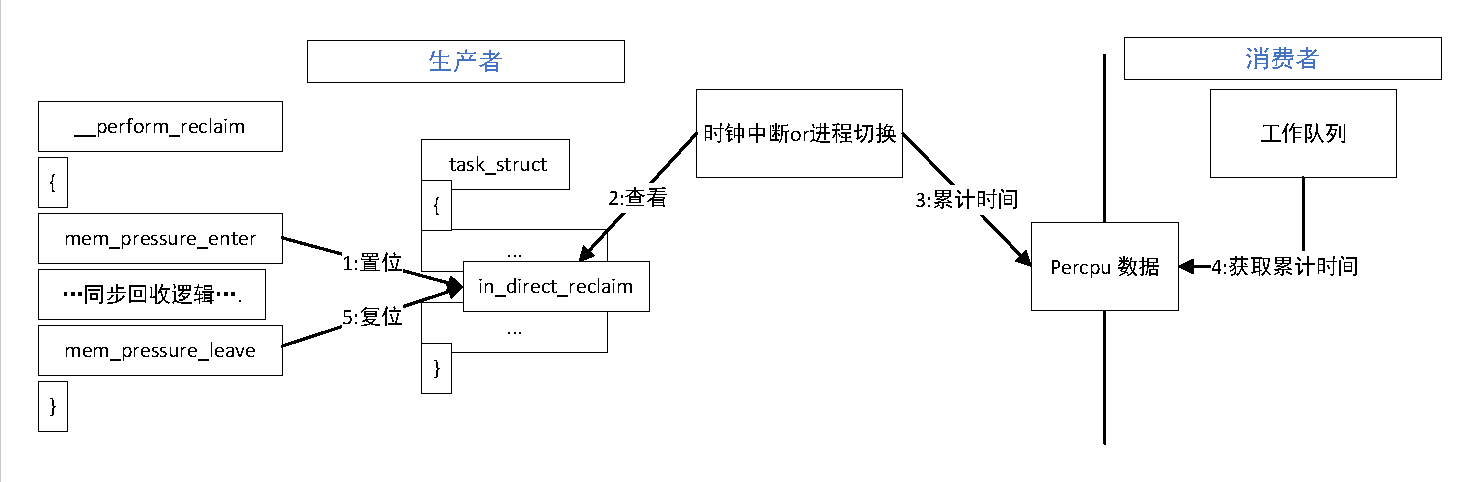
\includegraphics[width=\textwidth]{生产者和消费者.pdf}
    \caption{生产者消费者架构图}
    \label{fig:producer-consumer}
\end{figure}

系统实现如\ref{fig:producer-consumer}, 采用生产者-消费者模式构建内存压力实时监控与评估框架。该模式通过解耦数据采集与数据处理两个核心功能模块。生产者模块负责采集内存回收过程中的时间片数据,而消费者模块则周期性地处理这些数据,计算内存压力指标。临界区成员是Per-cpu中的数据,他统计了每个CPU中发生内存同步回收的时间。具体的信息详见\ref{tab:sensor_data}。同时我们在 Linux 中 task\_struct 中 in\_mem\_mempressure 表示这个进程在处同步内存回收了。

\begin{table}[htbp]
    \centering
    \caption{Per-cpu 变量}
    \label{tab:sensor_data}
    \begin{tabular}{ccc}
        \toprule
        成员名称& 数据类型     & 描述                                        \\ \midrule
        in\_direct\_reclaim & bool & 当前CPU是否处于同步内存回收状态\\
        \midrule
        time & u32 & 上一次累积时间的时间戳\\
        \midrule
        total\_time &u32&当前CPU处于同步内存回收状态的累积时间\\
        \midrule
        total\_time\_prev&u32&上一次统计时CPU处于同步内存回收状态的累积时间\\
        \midrule
        total\_work\_time&u32&当前CPU处于工作状态的累积时间\\
        \midrule
        total\_work\_time\_prev&u32&上一次统计时CPU处于工作状态的累积时间\\
        \bottomrule
    \end{tabular}
  \end{table}

生产者模块的核心功能是精确捕获内核中与内存回收相关的状态切换时间信息。为实现这一目标,生产者在同步内存回收的起始和结束时刻改变状态。具体而言,当系统发生直接内存回收时,即进程在分配内存时因内存不足而触发同步回收操作,生产者立即改变状态。当同步回收过程结束,进程恢复正常执行时,生产者再次改变状态,并计算累积时间。同时每次时钟中断的时候,他会进行累积时间。初次之外,我们需要和调度系统交互,用来控制时钟中断收集间隔,因为当这个线程调度出去的时候,CPU就不会花费时间来处理同步内存回收,当调度进来的时候,我们就需要重新计算,所以需要和调度系统交互并且在task\_struct中in\_mem\_mempressure标志来表示这个线程是否在处理同步内存回收。

消费者模块使用工作对列来实现,周期的从Per-cpu中读取读取,进行聚合,在\ref{sec:工作队列}介绍了选用工作队列的原因,在\ref{sec:内存压力计算算法}中介绍了具体的算法。


\subsection{生产者工作流程}

图\ref{fig:time-ticker} 所示为时钟中断处理流程。该流程始于时钟中断的触发,随后系统读取当前CPU的Per-CPU变量,并进入一个关键判定节点:判断in\_direct\_reclaim标志的状态。

若in\_direct\_reclaim为真,表明当前CPU正处于直接内存回收(direct reclaim)状态。此时,系统会执行以下操作:首先,通过cpu\_clock(cpu)函数获取当前时间戳,记为now;其次,计算时间差(now - time),并将其累加到total\_time变量中,用于统计同步内存回收所消耗的时间;最后,将now的值赋给time,以更新当前时间记录。这一过程确保了系统能够准确记录CPU在同步内存回收上花费的时间。

若in\_direct\_reclaim为假,则表明当前CPU未处于直接内存回收状态。此时,系统会计算时间差(now - time),并将其累加到total\_work\_time变量中,用于统计CPU在工作状态下的时间消耗。无论in\_direct\_reclaim的真假,流程最终都会汇聚至结束节点,完成一次时钟中断的处理。

\begin{figure}[h]
    \centering
    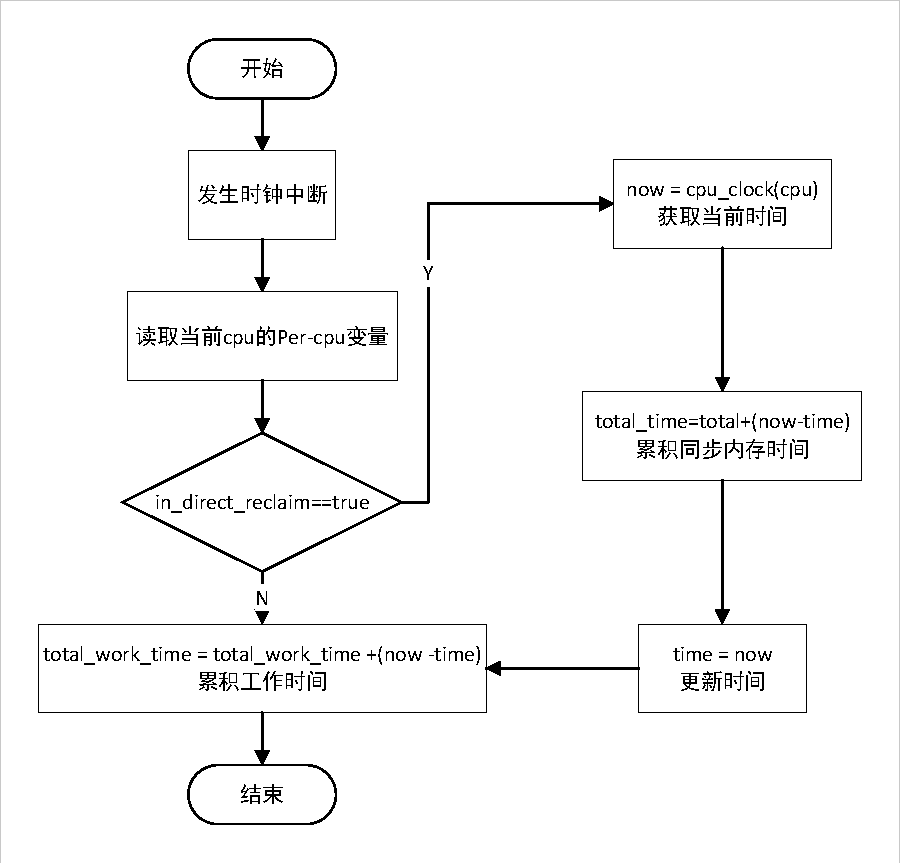
\includegraphics[width=\textwidth]{时钟中断.pdf}
    \caption{时钟中断流程图}
    \label{fig:time-ticker}
\end{figure}


此外,在进程切换时,系统会检查task\_struct中的in\_mem\_mempressure标志。如果当前进程的in\_mem\_mempressure为true,则表明该进程涉及内存压力,此时需要修改Per-CPU变量中的in\_direct\_reclaim标志,以表示当前CPU不再花费时间进行同步内存回收。反之,如果要切换进来的进程的in\_mem\_mempressure为true,则需要将Per-CPU变量中的in\_direct\_reclaim标志设置为true,表示当前CPU需要花费时间进行同步内存回收。


\subsection{工作队列}
\label{sec:工作队列}

工作队列(Workqueue)是Linux内核中用于异步任务处理的重要机制,其设计初衷是为需要在进程上下文中执行的任务提供一种高效且可靠的调度方式。在内存压力监控的实现中,工作队列的选用基于其独特的设计优势,能够满足复杂统计任务的需求。内存压力的计算是一个复杂的统计过程,涉及多个步骤:首先需要获取互斥锁以保护共享数据,随后进行较长时间的数据处理。这类操作必须在进程上下文中执行,因为它们可能会引起睡眠,而中断上下文则无法满足这一要求。此外,内存压力的监控需要周期性执行,以实时跟踪系统状态的变化。工作队列提供的延迟执行机制(如queue\_delayed\_work)正好契合这一需求。同时,由于内存压力的计算主要用于系统监控和决策支持,对实时性要求相对较低,因此可以容忍一定程度的执行延迟。

工作队列作为Linux内核中经过充分验证的标准机制,为异步任务的执行提供了可靠的保障。其主要功能特性包括任务调度、周期补偿和资源优化。工作队列能够确保任务在合适的时机得到执行,并在系统负载较高时自动调节执行频率。对于周期性的监控任务,工作队列实现了完善的补偿机制。即使在系统负载较高导致某些统计周期被延迟时,也能通过计算错过的周期数并进行相应补偿,确保监控数据的连续性和准确性。此外,工作队列的共享特性使其能够根据系统状态动态调整任务执行频率。当系统处于空闲状态时,任务会自动停止,避免不必要的资源消耗;当系统负载升高时,任务执行频率会自动调节,确保内存压力监控不会对系统性能造成显著影响。

如果采用专用内核线程来实现内存压力监控功能,开发者需要手动处理线程的创建、销毁和唤醒,同时还需考虑各种边界情况,如系统负载过高时的处理策略、错过统计周期的补偿机制等。这些工作不仅增加了代码的复杂度,也提高了出错的可能性。在内核编程中,边界条件的处理往往是最容易出现问题的地方,而这类问题通常难以重现和调试。相比之下,工作队列已经为这些复杂的情况提供了完善的处理机制,使得开发者可以专注于内存压力计算的核心逻辑实现。

表\ref{tab:workqueue_api}总结了工作队列相关的主要API及其功能。
\begin{table}[htbp]
\centering
\caption{工作队列相关API}
\label{tab:workqueue_api}
\begin{tabular}{cc}
\toprule
\textbf{API} & \textbf{功能描述} \\
\midrule
alloc\_workqueue & 创建一个新的工作队列 \\
\midrule
destroy\_workqueue & 销毁工作队列 \\
\midrule
INIT\_WORK & 初始化普通工作 \\
\midrule
INIT\_DELAYED\_WORK & 初始化延迟工作 \\
\midrule
queue\_work & 将任务加入到工作队列 \\
\midrule
queue\_delayed\_work & 延迟执行任务 \\
\bottomrule
\end{tabular}
\end{table}
% //!这里需要修改,加上一个工作队列工作的图,就是怎么进行循环工作的
综上所述,工作队列凭借其成熟的任务调度机制、周期补偿功能以及资源优化特性,为内存压力监控提供了一个稳定可靠的执行环境。其标准化的API接口和自动化的边界处理机制,显著降低了开发复杂度,同时提高了系统的健壮性和可维护性。


\subsection{临界区的保护}

在生产者-消费者模型中,生产者负责采集内存回收过程中的累积时间,而消费者(工作队列)则负责处理这些数据,计算并输出内存压力指标。为了确保数据在并发环境下的完整性和一致性,同时兼顾性能,需要对临界区进行精细的保护。

在详细阐述临界区保护策略之前,简要介绍本研究所采用的核心同步机制:序列锁(Seqlock)。序列锁是 Linux 内核提供的一种轻量级同步原语,特别适用于读多写少且写操作简短的场景。其基本原理如图 \ref{fig:seqlock} 所示。序列锁维护一个序列计数器,写操作通过递增该计数器来标识数据更新的开始和结束(奇数表示写操作进行中,偶数表示无写操作)。读操作在开始时记录序列号 read\_seqbegin() ,并在读取完成后再次检查序列号 read\_seqretry() 。如果序列号发生变化,则表明在读取过程中发生了写操作,读操作需要重试,以确保读取到一致的数据。

\begin{figure}[H]
    \centering
    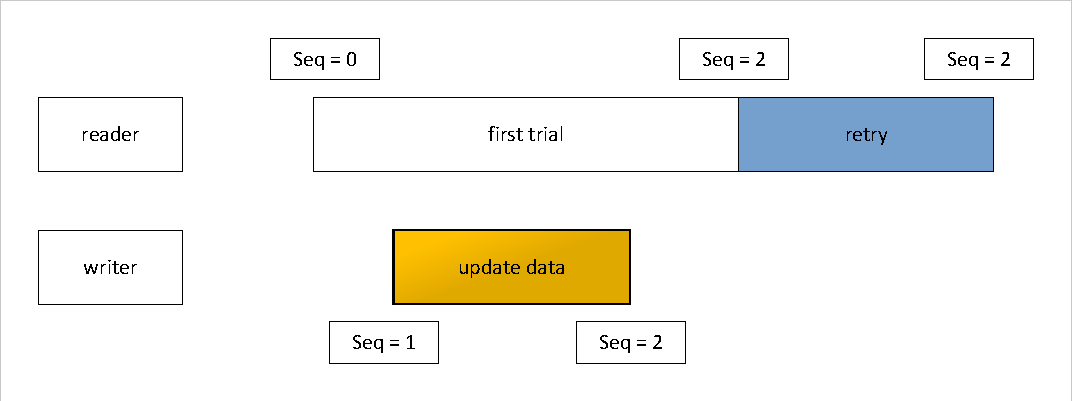
\includegraphics[width=\textwidth]{seqlock.pdf}
    \caption{序列锁(Seqlock)原理示意图}
    \label{fig:seqlock}
\end{figure}

该方案的选择主要基于以下多维约束分析:

\begin{enumerate}
    \item \textbf{per-CPU 数据:} 每个 CPU 核心维护一份独立的数据结构,在表\ref{tab:sensor_data}中可以看到存储了CPU的统计信息。虽然 per-CPU 变量在更新时本身具有原子性,无需额外加锁,但考虑到消费者需要读取所有 CPU 的 per-CPU 数据进行聚合计算,因此仍需采取适当的同步措施。

    \item \textbf{全局统计信息:} 一个全局静态变量,用于存储所有 CPU 停顿时间的累加值,以及用于平滑计算的历史统计数据。该变量的访问涉及多个 CPU 的数据聚合,因此需要严格的保护。

    \item \textbf{\texttt{task\_struct->in\_mem\_mempressure} 标志:} 进程描述符(\texttt{task\_struct})中的一个标志位,用于标识当前进程是否涉及内存压力。用于指导每次进程切换的时候,是否需要更新Per-CPU中的in\_direct\_reclaim标志。
\end{enumerate}

基于以上数据结构的特点和访问模式,本研究采用了如下的临界区保护策略:

\begin{itemize}
    \item \textbf{per-CPU 数据中的累计时间采用序列锁(Seqlock)保护。}
    \begin{itemize}
        \item 选择序列锁的主要原因是时钟中断处理函数需要更新该数据,而时钟中断处理函数不能阻塞。
        \item per-CPU 数据结构简单,通常为 32 位或 64 位无符号整型,写操作(累加时间)非常快速,且读取时可以整体复制,满足序列锁的使用条件。
        \item 由于内存同步回收通常不是频繁事件,因此对停顿时间的累加操作相对较少,属于典型的读多写少场景,与序列锁的设计理念高度契合。
    \end{itemize}

    \item \textbf{全局统计信息采用互斥锁(Mutex)保护。} 互斥锁提供了更强的互斥性,适用于保护涉及较长时间计算或复杂数据结构的操作。全局统计信息的更新涉及多个 CPU 数据的聚合和历史数据的平滑计算,操作相对耗时,因此采用互斥锁可以确保数据的一致性和完整性。

    \item \textbf{\texttt{task\_struct->in\_direct\_reclaim} 标志的访问由运行队列锁(Runqueue Lock)隐式保护。}
    该标志在同步内存回收开始时置位,在结束时复位。在置位和复位操作期间,内核会持有相应 CPU 的运行队列锁,并关闭本地中断,这可以防止其它 CPU 或中断对当前进程的调度产生干扰。而在时钟中断处理函数中检查该标志时,由于持有运行队列锁可以保证当前进程不会被调度到其它 CPU,因此直接访问该标志是安全的,无需额外的锁保护。这种利用已有锁机制进行保护的方式,避免了引入新的锁,降低了系统的复杂度和开销。
\end{itemize}

通过上述针对性的临界区保护策略,本框架在确保数据一致性的前提下,最大限度地降低了同步开销,提升了系统的整体性能。


\subsection{内存压力计算算法}
\label{sec:内存压力计算算法}


\SetKwFunction{FixedPowerInt}{fixed\_power\_int}
\SetKwProg{Fn}{Function}{:}{}
\begin{algorithm}[H]
    \caption{Helper Functions}
    \label{alg:helper_functions}
    \SetKwFunction{FixedPowerInt}{fixed\_power\_int}
    \SetKwProg{Fn}{Function}{:}{}

    \Fn{\FixedPowerInt(\(x\), \(n\))}{  % x: 定点数 (Q0.10), n: 非负整数
        \(result \gets 2^{10}\) \;  \tcp*[l]{初始化为 1.0,定点数}
        \If{\(n > 0\)}{
            \While{\(true\)}{
                \If{\((n \land 1) \neq 0\)}{  % 如果 n 是奇数
                    \(result \gets (result \times x + 2^9) \gg 10\)\; \tcp*[l]{累乘 x, 保持定点数}
                }
                \(n \gets n \gg 1\)\;  \tcp*[l]{n 右移一位 (除以 2)}
                \If{\(n = 0\)}{\textbf{break}}  % 如果 n 变为 0,退出循环
                \(x \gets (x \times x + 2^9) \gg 10\)\; \tcp*[l]{x 自乘, 保持定点数}
            }
        }
        \Return \(result\)\;  % 返回 x^n (定点数)
    }
\end{algorithm}






\begin{algorithm}[H]
    \caption{Memory Pressure Sampling \& Update (Optimized)}
    \label{alg:mem_pressure_optimized}
    \SetAlgoLined
    \DontPrintSemicolon

    \Input{
        \begin{varwidth}{\linewidth}
            \(\text{total\_time}_i, \text{total\_time\_prev}_i, \text{total\_work\_time}_i, \text{total\_work\_time\_prev}_i\)\\
            (for each CPU \(i\));\\
            \(\text{mem\_pressure\_time}, \text{mem\_pressure\_time\_prev}\),\\
            \(\text{mem\_pressure\_prev}, \text{next\_update\_time}, \text{last\_update\_time}, T, \text{exp}\);
        \end{varwidth}
    }
    \Output{updated \(\text{mem\_pressure\_prev}, \text{mem\_pressure\_time\_prev}, \text{next\_update\_time}, \)\\
    \(\text{last\_update\_time}\)}

    \BlankLine

    \(\text{weight\_pressure\_time}, \text{work\_time} \gets \text{calculate\_weighted\_pressure\_time}(\text{cpu\_data})\)\;
    \(\text{mem\_pressure\_time} \gets \lfloor \text{weight\_pressure\_time}/\max(\text{work\_time},1)\rfloor\)\;

    \(\text{next\_update\_time}, \text{last\_update\_time}, \text{missed}, \text{period} \gets\) \(\text{update\_timestamps}(\text{sched\_clock}(), \text{next\_update\_time}, \text{last\_update\_time}, T)\)\;

    \(\text{mem\_pressure\_prev} \gets \text{exponential\_smoothing}(\)
    \qquad \(\text{mem\_pressure\_time}, \text{mem\_pressure\_time\_prev},\)
    \qquad \(\text{period}, \text{mem\_pressure\_prev}, \text{exp}, \text{missed})\)\;
\end{algorithm}

\begin{algorithm}[H]
\caption{calculate\_weighted\_pressure\_time}
\label{alg:calculate_weighted_pressure_time}
\SetAlgoLined
\DontPrintSemicolon
\Input{\(\text{total\_time}_i, \text{total\_time\_prev}_i, \text{total\_work\_time}_i, \text{total\_work\_time\_prev}_i\)\\
(for each CPU \(i\));\\}
\Output{\(\text{weight\_pressure\_time}, \text{work\_time}\)}
\(\text{weight\_pressure\_time} \gets 0,\quad \text{work\_time} \gets 0\)\;
\For{each CPU \(i\)}{
    \(\text{weight\_pressure\_time} \gets \text{weight\_pressure\_time} + (\text{total\_time}_i - \text{total\_time\_prev}_i) \times (\text{total\_work\_time}_i - \text{total\_work\_time\_prev}_i)\)\;
    \(\text{work\_time} \gets \text{work\_time} + (\text{total\_work\_time}_i - \text{total\_work\_time\_prev}_i)\)\;
}
\Return{\(\text{weight\_pressure\_time}, \text{work\_time}\)}
\end{algorithm}

\begin{algorithm}[H]
\caption{update\_timestamps}
\label{alg:update_timestamps}
\SetAlgoLined
\DontPrintSemicolon
\Input{\(\text{now}, \text{next\_update\_time}, \text{last\_update\_time}, T\)}
\Output{ \(\text{next\_update\_time}, \text{last\_update\_time}, \text{missed}, \text{period}\)}
\If{\(\text{now} < \text{next\_update\_time}\)}{
\Return{\(\text{next\_update\_time}, \text{last\_update\_time}, 0, 0\)}
}
\(\text{missed} \gets \lfloor(\text{now}-\text{next\_update\_time})/T\rfloor\)\;
\(\text{next\_update\_time} \gets \text{next\_update\_time} + (\text{missed}+1) \times T\)\;
\(\text{period}\gets \text{now}-\text{last\_update\_time}\)\;
 \(\text{last\_update\_time}\gets \text{now}\)\;
\Return{\(\text{next\_update\_time}, \text{last\_update\_time}, \text{missed}, \text{period}\)}
\end{algorithm}

\begin{algorithm}[H]
\caption{exponential\_smoothing}
\label{alg:exponential_smoothing}
\SetAlgoLined
\DontPrintSemicolon
\Input{
    \begin{varwidth}{\linewidth}
      \(\text{mem\_pressure\_time}, \text{mem\_pressure\_time\_prev}, \text{period}\)\\
      \(\text{mem\_pressure\_prev}, \text{exp}, \text{missed}\)
    \end{varwidth}
}
\Output{\(\text{mem\_pressure\_prev}\)}

\(\text{sample\_time}\gets \text{mem\_pressure\_time}-\text{mem\_pressure\_time\_prev}\)\;
    \If{\(\text{sample\_time}>\text{period}\)}{
        \(\text{sample\_time}\gets \text{period}\)
    }
    \(\text{mem\_pressure\_time\_prev} \gets \text{mem\_pressure\_time\_prev} + \text{sample\_time}\)\;
    \(\text{tmp\_mem\_pressure}\gets \lfloor(\text{sample\_time}\times 100\times 2^{10})/\text{period}\rfloor\)\;
    \If{\(\text{missed}>0\)}{
      \(\text{exp} \gets \text{exp}^{\text{missed}}\)
    }
    \(\text{new\_mem\_pressure}\gets \text{mem\_pressure\_prev}\times \text{exp} + \text{tmp\_mem\_pressure}\times(2^{10}-\text{exp})\)\;
    \If{\(\text{mem\_pressure\_prev}>\text{tmp\_mem\_pressure}\)}{
      \(\text{new\_mem\_pressure} \gets \text{new\_mem\_pressure} + (2^{10}-1)\)
    }
    \(\text{mem\_pressure\_prev}\gets \lfloor \text{new\_mem\_pressure}/2^{10}\rfloor\)\;
    \Return{\(\text{mem\_pressure\_prev}\)}
\end{algorithm}



算法\ref{alg:helper_functions}中的FixedPowerInt(x, n)函数是实现定点数下的二进制快速幂计算。其主要作用是计算 \(x^n\) 的值,其中 \(x\) 是定点数,\(n\) 是非负整数。该函数通过二进制快速幂算法来高效计算幂。

\begin{itemize}
    \item \(\textbf{Line 3}\):初始化 \(\textit{result}\) 为 \(2^{10}\),即定点数表示下的1.0(Q0.10)。
    \item \(\textbf{Line 4-5}\):若 \(n = 0\),直接返回1.0;否则进入计算循环。
    \item \(\textbf{Line 6-11}\):在循环过程中,每次检查 \(n\) 的最低位:
        \begin{itemize}
            \item 如果最低位为1,则将当前的 \(\textit{result}\) 乘以 \(x\),并在乘法后加上 \(2^9\) 再右移10位,以保证保持定点数格式。
            \item 每次将 \(n\) 右移一位,若 \(n\) 变为0,则退出循环;否则将 \(x\) 自乘,得到 \(x^2\),并继续循环。
        \end{itemize}
    \item 最终返回计算得到的 \(\textit{result}\),即定点数形式的 \(x^n\)。
\end{itemize}

算法\ref{alg:mem_pressure_optimized}中的calculate\_weighted\_pressure\_time(cpu\_data)函数的主要作用是计算 CPU 的加权内存压力时间。通过遍历每个 CPU 的回收时间和工作时间,计算加权后的内存压力时间以及总的工作时间。

\begin{itemize}
    \item \(\textbf{Line 1}\):初始化 weight\_pressure\_time 和 work\_time 为 0。
    \item \(\textbf{Line 2-4}\):遍历每个 CPU,计算每个 CPU 的回收时间增量(tmp\_time)和工作时间增量(tmp\_work\_time),并将它们的乘积累加到 weight\_pressure\_time 中。同时,累加每个 CPU 的工作时间到 work\_time。
    \item 最终返回加权后的压力时间 weight\_pressure\_time 和总工作时间 work\_time。
\end{itemize}

算法\ref{alg:update_timestamps}中的update\_timestamps(now, next\_update\_time, last\_update\_time, T)函数用于更新采样时间戳,确保采样周期的正确性,并处理由于错过周期而导致的时间偏移。

\begin{itemize}
    \item \(\textbf{Line 1}\):获取当前时钟(`now`)。
    \item \(\textbf{Line 2}\):检查当前时刻是否小于下次更新时间(`next\_update\_time`)。如果小于,则表示尚未到达采样时间,直接返回。
    \item \(\textbf{Line 3-5}\):若当前时间距离下次更新时间的间隔超过了采样周期 \(T\),则计算错过的周期数(`missed`)。如果没有错过周期,则 `missed` 为0。
    \item \(\textbf{Line 6}\):更新下次更新时间 `next\_update\_time` 为下一个采样周期的时间点。
    \item \(\textbf{Line 7}\):计算当前时刻与上次更新时间(last\_update\_time)之间的周期 period,并更新 last\_update\_time 为当前时间。
    \item 返回更新后的 next\_update\_time、last\_update\_time、missed 和 period。
\end{itemize}

算法\ref{alg:exponential_smoothing}中的exponential\_smoothing函数实现了指数平滑(Exponential Smoothing)更新内存压力。该函数根据当前的内存压力时间、前一次的压力时间、当前采样周期、之前的内存压力和指数衰减系数,来计算新的内存压力。

\begin{itemize}
    \item \(\textbf{Line 1}\):计算当前的样本压力时间(sample\_time),即当前的 \\mem\_pressure\_time 减去前一次的 mem\_pressure\_time\_prev。
    \item \(\textbf{Line 2}\):如果 sample\_time 大于采样周期 period,则将 sample\_time 限制为 period,避免采样时间超出采样周期。
    \item \(\textbf{Line 3}\):更新前一次的内存压力时间 mem\_pressure\_time\_prev,将当前的 sample\_time 累加到 mem\_pressure\_time\_prev 中。
    \item \(\textbf{Line 4}\):将 sample\_time 转换为定点数表示的内存压力(tmp\_mem\_pressure),并确保其在合理范围内(0-100\%)。
    \item \(\textbf{Line 5}\):如果错过了采样周期(missed > 0),则更新指数衰减系数 exp。
    \item \(\textbf{Line 6}\):使用指数衰减系数 exp 和当前的 mem\_pressure\_prev 来计算新的内存压力 new\_mem\_pressure,并结合 tmp\_mem\_pressure 进行平滑更新。
    \item \(\textbf{Line 7}\):如果当前的 mem\_pressure\_prev 大于 tmp\_mem\_pressure,则进行微调,确保新的内存压力不会小于当前压力。
    \item \(\textbf{Line 8}\):将更新后的 new\_mem\_pressure 除以 \(2^{10}\)(右移10位),并将其赋值给 mem\_pressure\_prev。
    \item 返回更新后的 mem\_pressure\_prev。
\end{itemize}
\section{本章小结}